

\section{Background}\label{sec:background}

This section describes the background of SSD-based In-Storage Computing (Section~\ref{sec:ISC_background}) and a Hadoop MapReduce framework (Section~\ref{sec:searchEngineArch}).

\subsection{In-Storage Computing (ISC)}\label{sec:ISC_background}
In-Storage Computing is a new computing paradigm, where a storage device play a major role in data processing as a computing node. Unlike the traditional CPU-centric computing model, nowadays non-CPU components such as storage devices or Graphical Processing Unit (GPU) can make a big contribution to data computation by using their computing capabilities~\cite{ActivFlash:FAST:2013,CUDA:Tutorial:2012,SmartSSD:SIGMOD:2013}, so-called '\emph{rebellion of peripherals against CPU}'.


\begin{figure}[htbp]
  \centering
  \begin{tabular}{ccc}
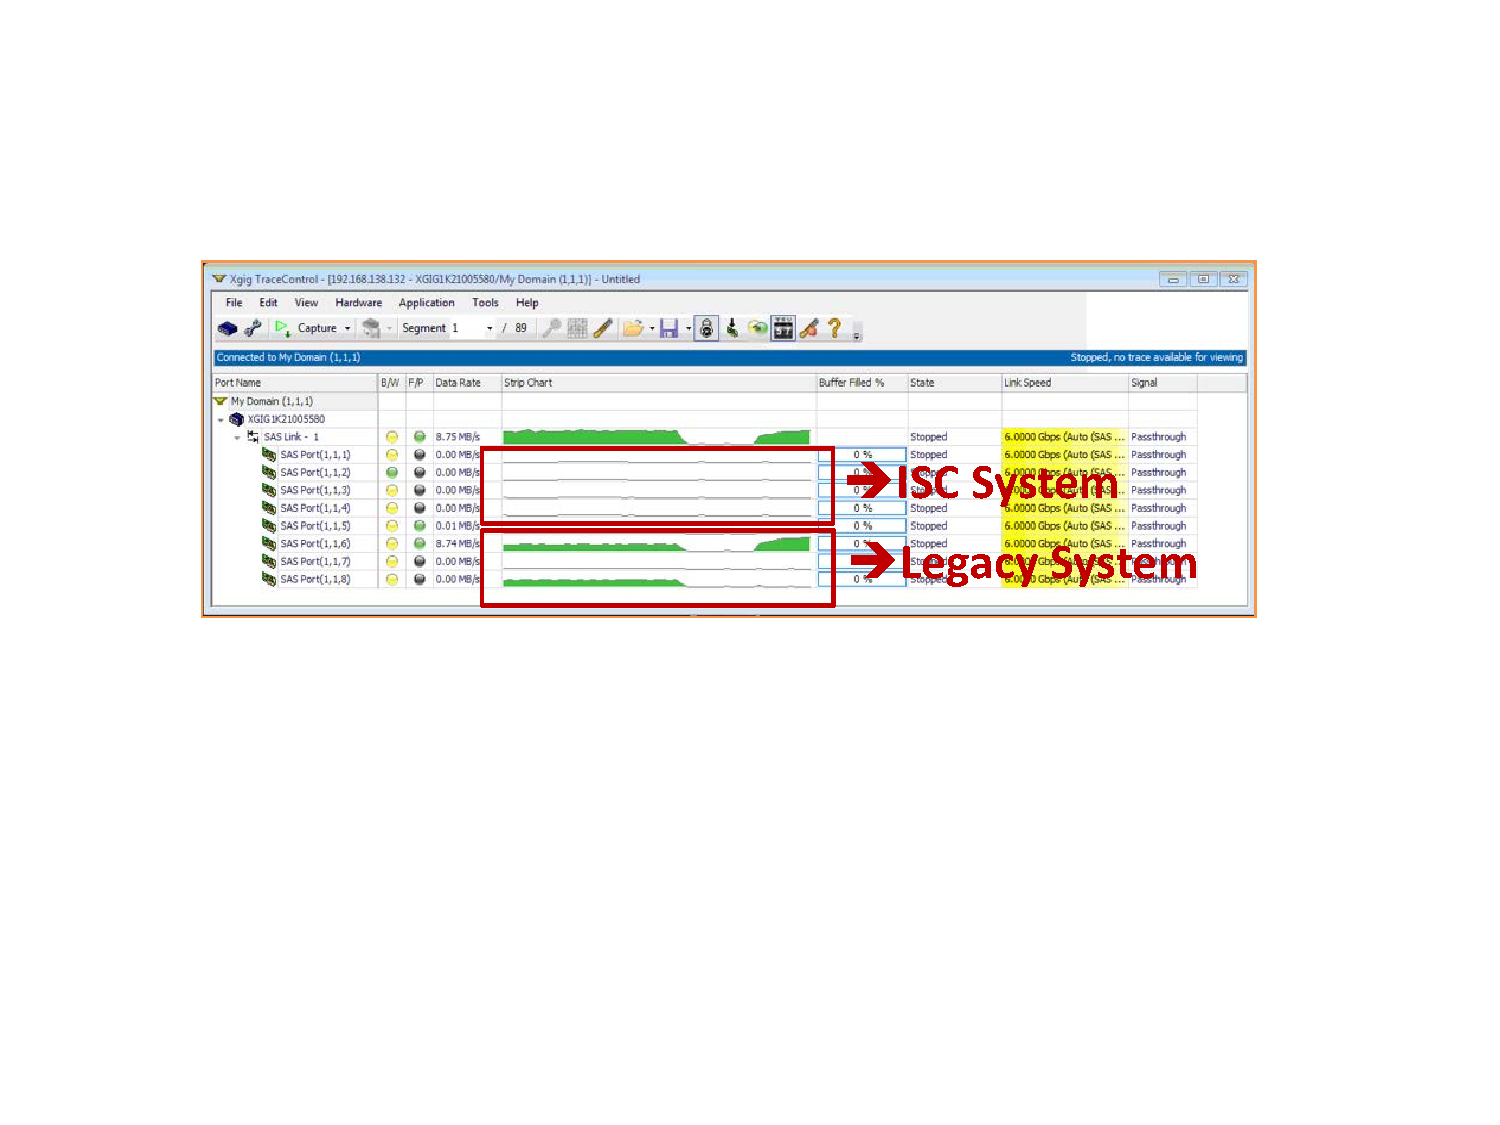
\includegraphics[width=0.99\columnwidth]{figures/Bus_Analyzer.pdf}
\end{tabular}
  \caption{The amount of data transfer from a device to a host. The upper most green bar corresponds to the total amount of data for both systems.}
  \label{fig:Bus_Alanyzer}
 \end{figure}


Figure~\ref{fig:Bus_Alanyzer} shows the amount of data transferring from a device (SSD) to a host system and we captured this with our 12Gbps SAS/SATA bus analyzer~\cite{BusAnalyzer:JDSU:techspec}. For this study, we set up two Hadoop systems (i.e., our proposed ISC Hadoop system and typical Hadoop system with SSDs) and connect them to the bus analyzer. Then, we run the same Hadoop application with identical data on both Hadoop systems at the same time. As shown in the figure, both exhibit a huge difference between our ISC model (upper rectangle) and the traditional CPU-centric computing model (lower rectangle). This clearly presents that the ISC system does not (or very rarely) transfer data to the host system for computation, while the legacy CPU-centric system keeps loading all the data to the host system (that is, host DRAM). All the main benefits of the ISC system originate from this factor.


Even though the main idea of ISC has been already proposed and implemented in the context of Hard Disk Drives (HDDs), it was not successfully adopted because of the still very limited computational capabilities of HDDs~\cite{Keeton1998,ActiveDisks:ASPLOS:1998}. However, the modern SSDs have been equipped with even stronger computing resources such as multi-core CPUs and DRAM so that people start to rethink of SSDs as another type of a computing unit, not just as a faster HDDs. 

SSDs typically provides a lot higher internal bandwidth (about 5$\times$ higher) than host I/O interface (SATA or SAS) bandwidth~\cite{SmartSSD:SIGMOD:2013,Minerva:De:2013}. The SSDs adopted for our ISC Hadoop system offers about 3.2GB/s of the aggregated internal bandwidth, while 750MB/s of host I/O interface bandwidth\footnote{\small Both are theoretical bandwidths and based on Samsung 6Gb SAS Enterprise SSD (400GB SLC).}. Thus, moving data from devices to a host results in a significant waste of the high internal bandwidth. 
In addition, the low I/O latency inside SSDs is another noticeable factor. A regular I/O operation is affected heavily by the entire OS stack which introduces extra overheads (e.g., context switching, interrupt, file system overhead, etc). However, the internal I/O latency in SSDs can avoid those OS software overheads. These factors implies that \emph{I/O intensive applications can significantly benefit from the ISC model} because, unlike CPU-centric computing system, ISC systems can make the best use of the high internal bandwidth and low internal I/O latency. 

SSDs, in general, are equipped with low power processors not only to save energy consumption but also to lower manufacturing costs. This factor results in an ambivalent value of ISC computing model. That is, the low power processor such as ARM processors can help ISC applications save energy consumption. On the other hand, it implies \emph{CPU computation intensive applications are not favorable to our current ISC computing model}.


\begin{figure}[htbp]
  \centering
  \begin{tabular}{ccc}
 %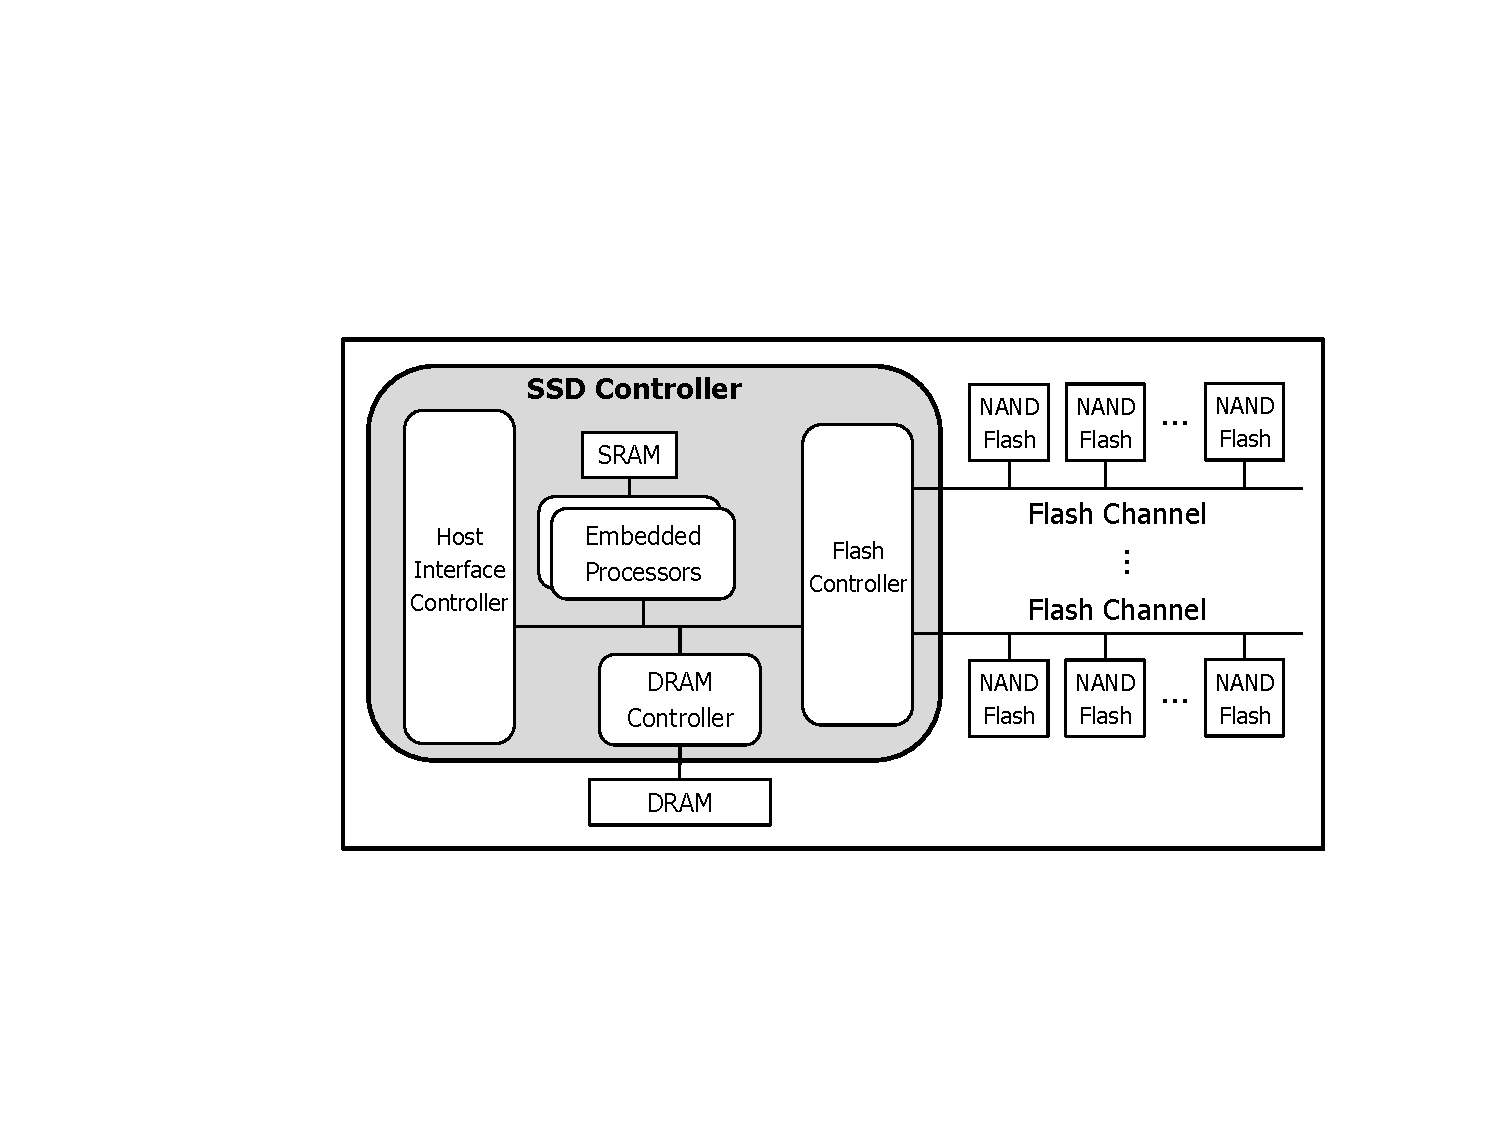
\includegraphics[width=0.95\columnwidth]{figures/SSDInternals.pdf}
 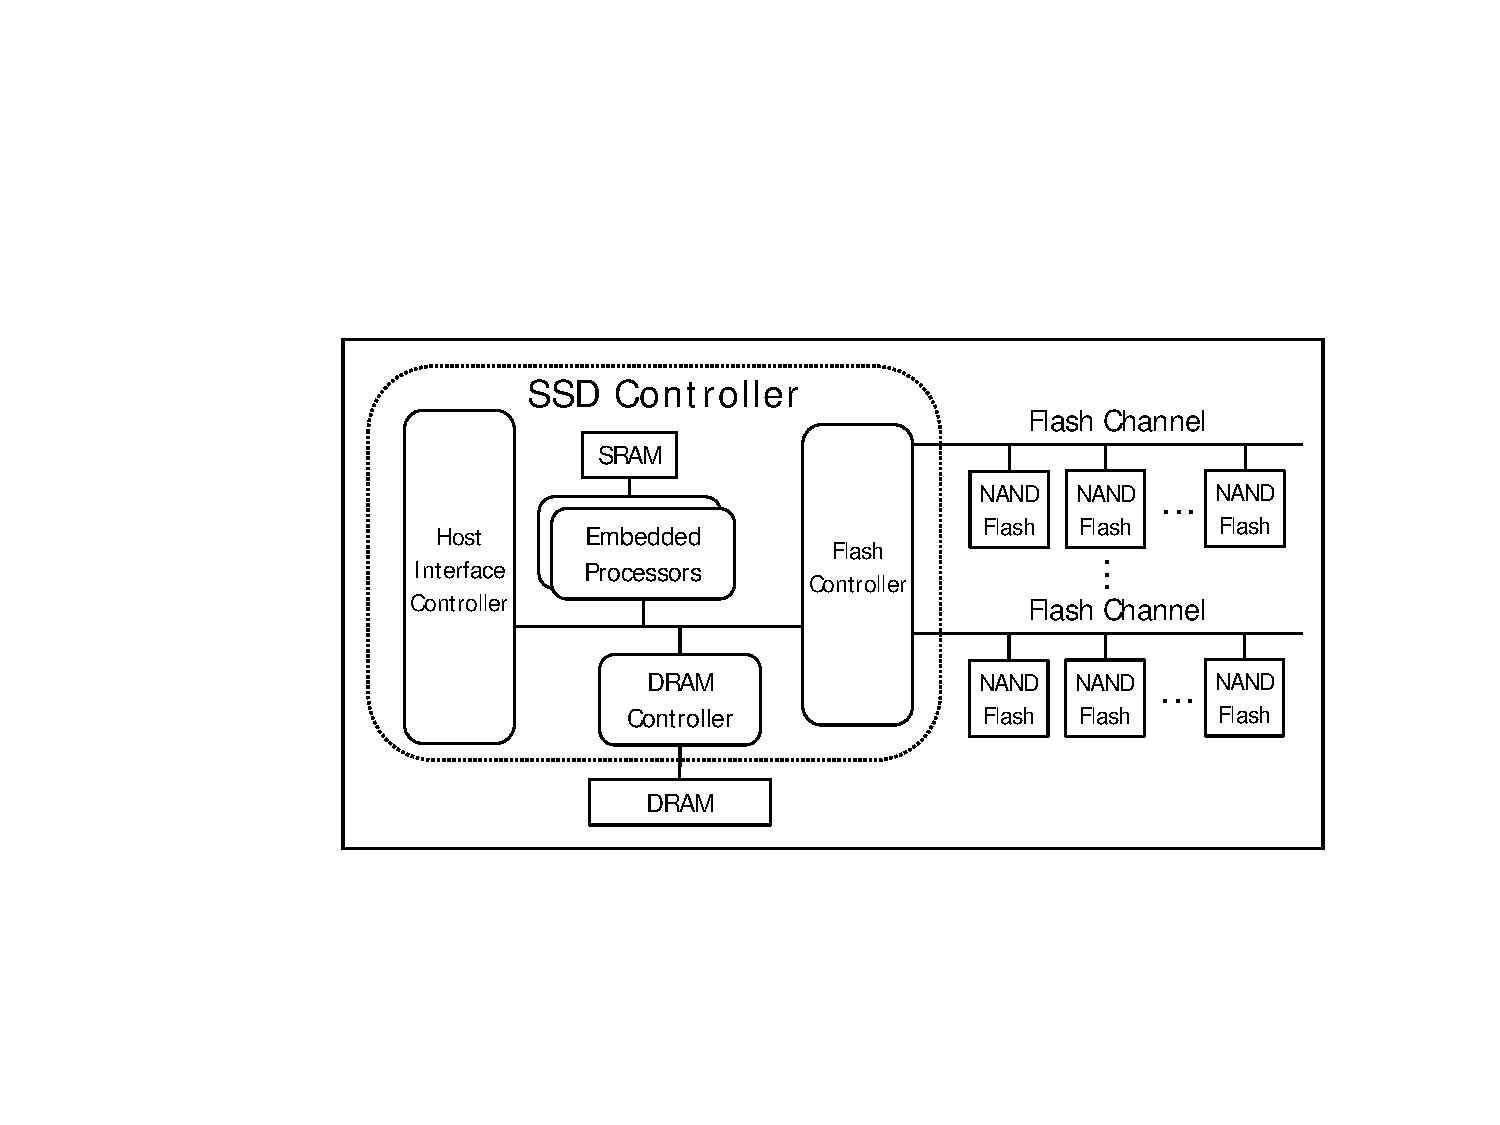
\includegraphics[width=0.99\columnwidth]{figures/ISC_HW_architecture.pdf}
\end{tabular}
  \caption{ISC hardware architecture}
  \label{fig:SSDInternals}
 \end{figure}


\subsubsection{ISC Hardware Architecture}\label{sec:SSDhw}
Figure~\ref{fig:SSDInternals} represents the hardware architecture of the modern SSD. The hardware architecture of our ISC SSD device is identical to regular SSDs.
%SSDs typically provides a lot higher internal bandwidth (about 5$\times$ higher) than host I/O interface (SATA or SAS) bandwidth~\cite{SmartSSD:SIGMOD:2013}. The SSDs adopted for ISC Hadoop framework offers about 3.2GB/s of the aggregated internal bandwidth, while 750MB/s of host I/O interface bandwidth\footnote{\small Both are theoretical bandwidths and based on Samsung 6Gb SAS Enterprise SSD (400GB SLC).}. This implies that moving data from devices to a host results in a significant waste of the high internal bandwidth. Unlike CPU-centric computing system, ISC systems can make the best use of this high internal bandwidth. 

An SSD is largely composed of NAND flash memory array, SSD controller, and (device) DRAM. The SSD controller is subdivided into four main subcomponents: host interface controller, embedded processors, DRAM controller, and flash controller.
The host interface controller processes commands from interfaces (typically SAS/SATA or PCIe) and distributes them to the embedded processors. Commands come from a user through the host I/O interface and the common interfaces are implemented by the host interface controller.
The embedded processors receive the commands and pass them to the flash controller. More importantly, they run SSD firmware codes for computation and execute Flash Translation Layer (FTL) for logical-to-physical address mapping~\cite{JSA:FTL:2009,CFTL:MASCOTS:2011}. Typically, the processor is a low-powered 32-bit processor such as an ARM processor. Each processor can have a tightly coupled memory (i.e., SRAM) to store performance-critical data or codes. Each processor can access DRAM through the DRAM controller. The flash controller controls data transfer between flash memory and DRAM.

%For data transfer between flash memory and DRAM, the Flash Controller, also called Flash Memory Controller (FMC), is adopted. The FMC runs Error Correction Code (ECC) and supports Direct Memory Access (DMA) functionality.

%The NAND flash memory package (also called chip) is persistent storage media and each package consists of one or more dies. The die is the smallest unit that can independently execute commands or report status. Each die contains one or more planes (usually one or two). Identical or concurrent operations can take place on each plane, although with some restrictions. Each plane subdivides into a number of blocks which are the smallest erase unit, and finally each block is composed of many pages (typically 64 or 128 pages)which are the smallest read/write unit.
The NAND flash memory package is the persistent storage media and each package is subdivided further into smaller units that can independently execute commands or report status.
An SSD is also equipped with a large size of DRAM for buffering data or storing metadata of the address mapping. All the flash channels share access to the DRAM. Thus, data transfer from the flash channels to the DRAM needs to be serialized~\cite{SmartSSD:SIGMOD:2013}.


%The Smart SSD ecosystem consists of both hardware (Section~\ref{sec:SSDhw}) and software components (Section~\ref{sec:softArch}) to execute user-defined programs.





\subsubsection{ISC Software Architecture}\label{sec:softArch}

%Smart SSDs, unlike the traditional CPU-centric computing systems, enable ISC devices to play a major role in computation by offloading key functions of host systems into ISC devices. Since its hardware architecture is identical to the aforementioned modern SSDs shown in Figure~\ref{fig:SSDInternals}, this section describes our Smart SSD software architecture and key components as ISC devices.

This section describes the system architecture and software key components for our ISC ecosystem including host system and storage device. Figure~\ref{fig:SmartSSD_arch} represents our ISC software architecture composed of two main components: \emph{ISC firmware} inside the SSD and \emph{ISC host program} in the host system. The ISC host program communicates with the ISC firmware through ISC Application Programming Interfaces (APIs).




\begin{figure}[tbp]
%\vspace{-5mm}
	\centering
		%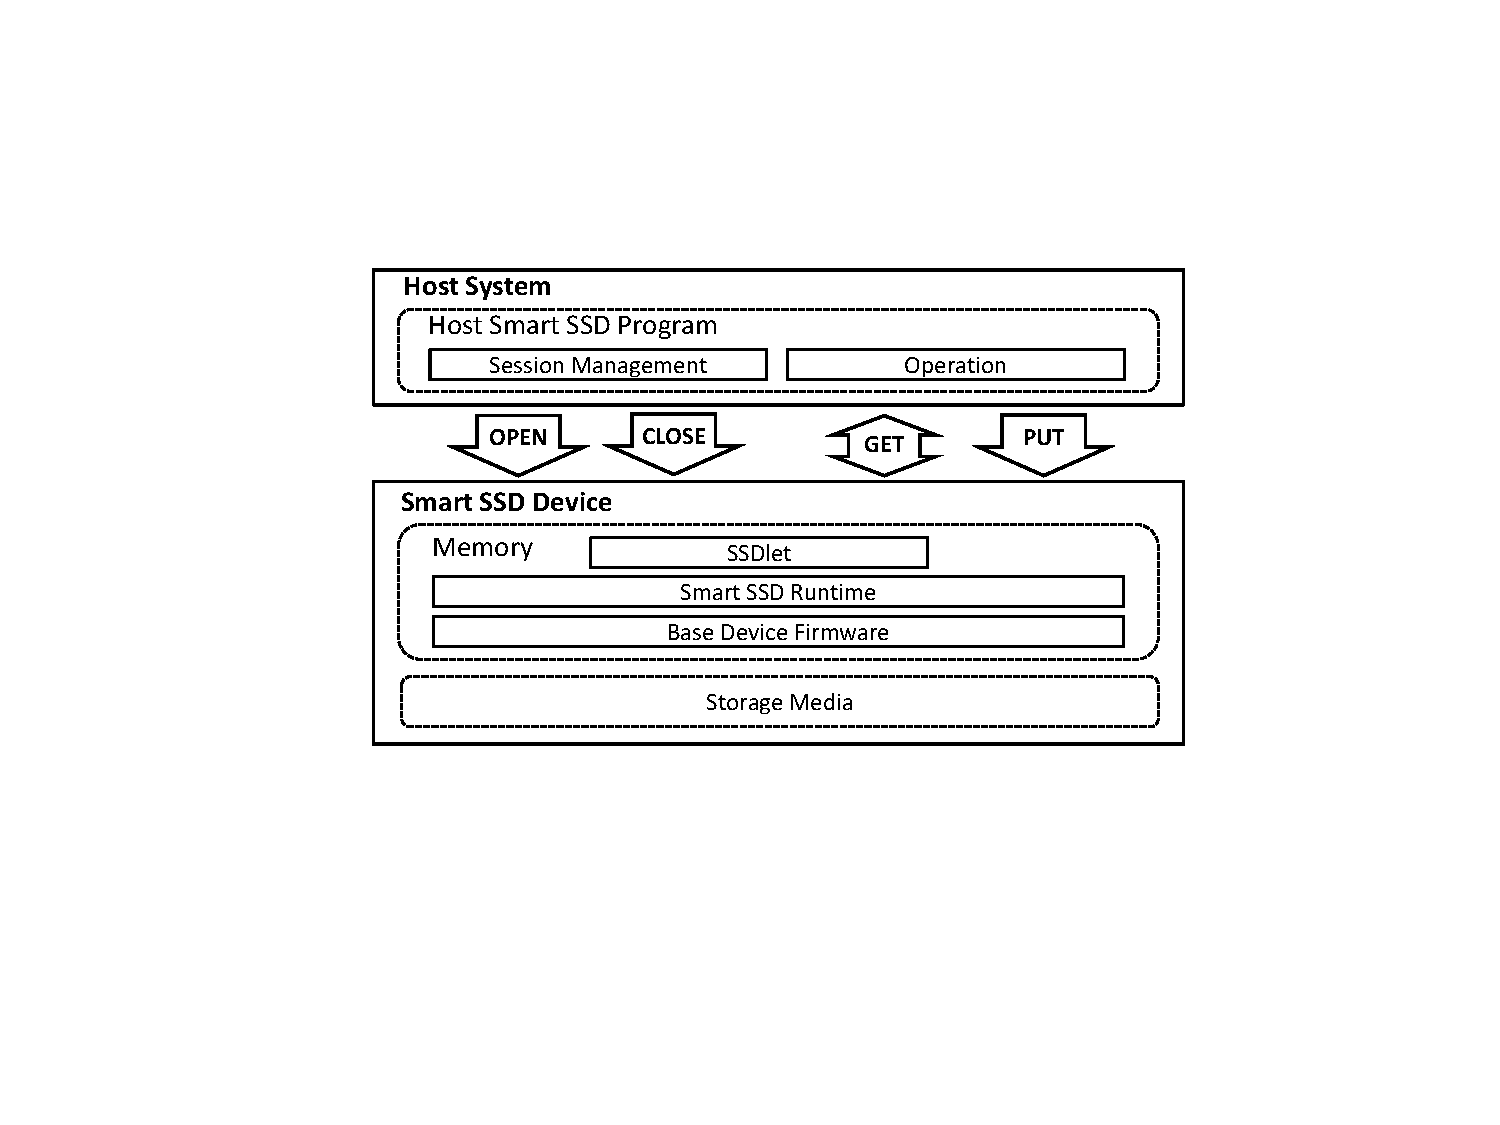
\includegraphics[width=0.95\columnwidth]{figures/SmartSSD_Architecture.pdf}
		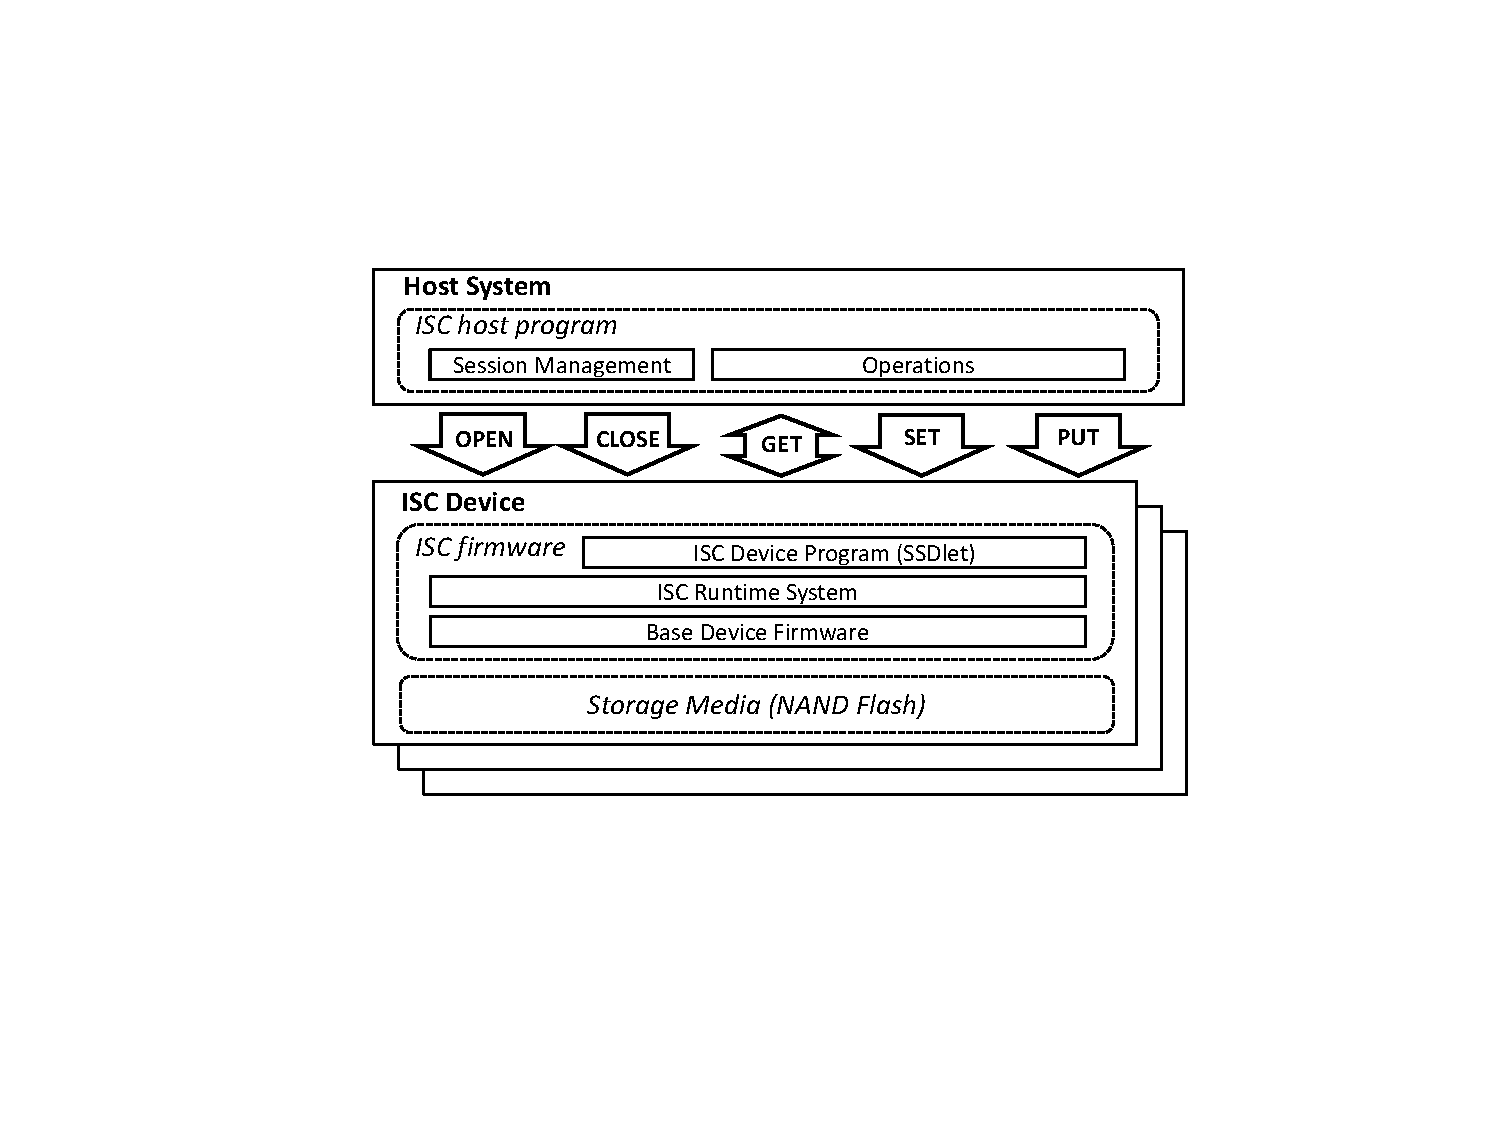
\includegraphics[width=0.99\columnwidth]{figures/ISC_SW_architecture.pdf}		
	\caption{ISC software architecture}
	\label{fig:SmartSSD_arch}
\end{figure}

%As illustrated in Figure~\ref{fig:SmartSSD_arch}, our Smart SSD consists of several key software components and it communicates with a Smart SSD host program via Smart SSD application programming models (APIs).

Since both a host system and an ISC storage device cooperatively compute data, we need to define two types of interactions (i.e., ISC host interface and ISC device interface) among a host, a device, and an ISC application. The ISC host interface is in charge of communication between the host and ISC devices to control ISP operations. The ISC device interface is on how the ISC runtime system in the storage device internally interacts with an ISC application in response to external inputs. A host ISC program implements the host interface logic, while a device ISC program (i.e., SSDlet) implements the device interface logic. We implement our ISC applications by using the ISC APIs.

The ISC firmware is subdivided into three sub-components: SSDlet, ISC runtime, and base device firmware.
An SSDlet is an ISC device program inside the SSD. It implements application logic and responds to the ISC host program. The SSDlet is executed in an event-driven manner by the ISC runtime system. An ISC runtime system connects the ISC device program with a base device firmware, and implements the library of ISC APIs. In addition, a base device firmware also implements normal I/O operations (read and write) of a storage device.

After the SSDlet is installed in the ISC device, a host system runs the ISC host program to interact with the SSDlet in the devices. This ISC host program consists largely of two components: a session management component and an operation component. The session component manages the lifetime of a session for ISC device applications so that the ISC host program can launch an SSDlet by opening a session to the ISC device. To support this session management, our ISC programming model provides two APIs, namely, OPEN and CLOSE. OPEN starts a session and CLOSE terminates a session. Once OPEN starts a session, the runtime resources such as memory and threads are assigned to run the SSDlet and a unique session ID is returned to the ISC host program. %This session ID must be associated to interact with the SSDlet afterwards. 
When CLOSE terminates the established session, it releases all the assigned resources and closes SSDlet associated with the session ID.

Once a session is established by OPEN, the operation component helps the ISC host program interact with SSDlet in an ISC device with GET, SET and PUT APIs. This GET operation is used to check the status of SSDlet and receive output results from the SSDlet if the results are ready. This GET API implements the polling mechanism of the SAS/SATA interface because, unlike PCIe, such traditional block devices cannot initiate a request to a host such as interrupts. 

Aside from the existing OPEN, GET, and CLOSE APIs, \emph{we implemented two more APIs: SET and PUT}. The SET operation delivers the new ISC metadata information (e.g., starting LBA, data length, etc.) from a host to an ISC device within a session. This SET API is very useful to process multiple non-contiguous data within one session. Without the SET API, we had to re-open another session after closing the previous session, which causes an extra overhead. PUT is also newly implemented to internally write data to the NAND flash media without help of a local file system. This API is useful to store the intermediate data during ISC processing.


\subsection{Hadoop MapReduce Framework}\label{sec:searchEngineArch}

\begin{figure}[htbp]
  \centering
  \begin{tabular}{ccc}
 %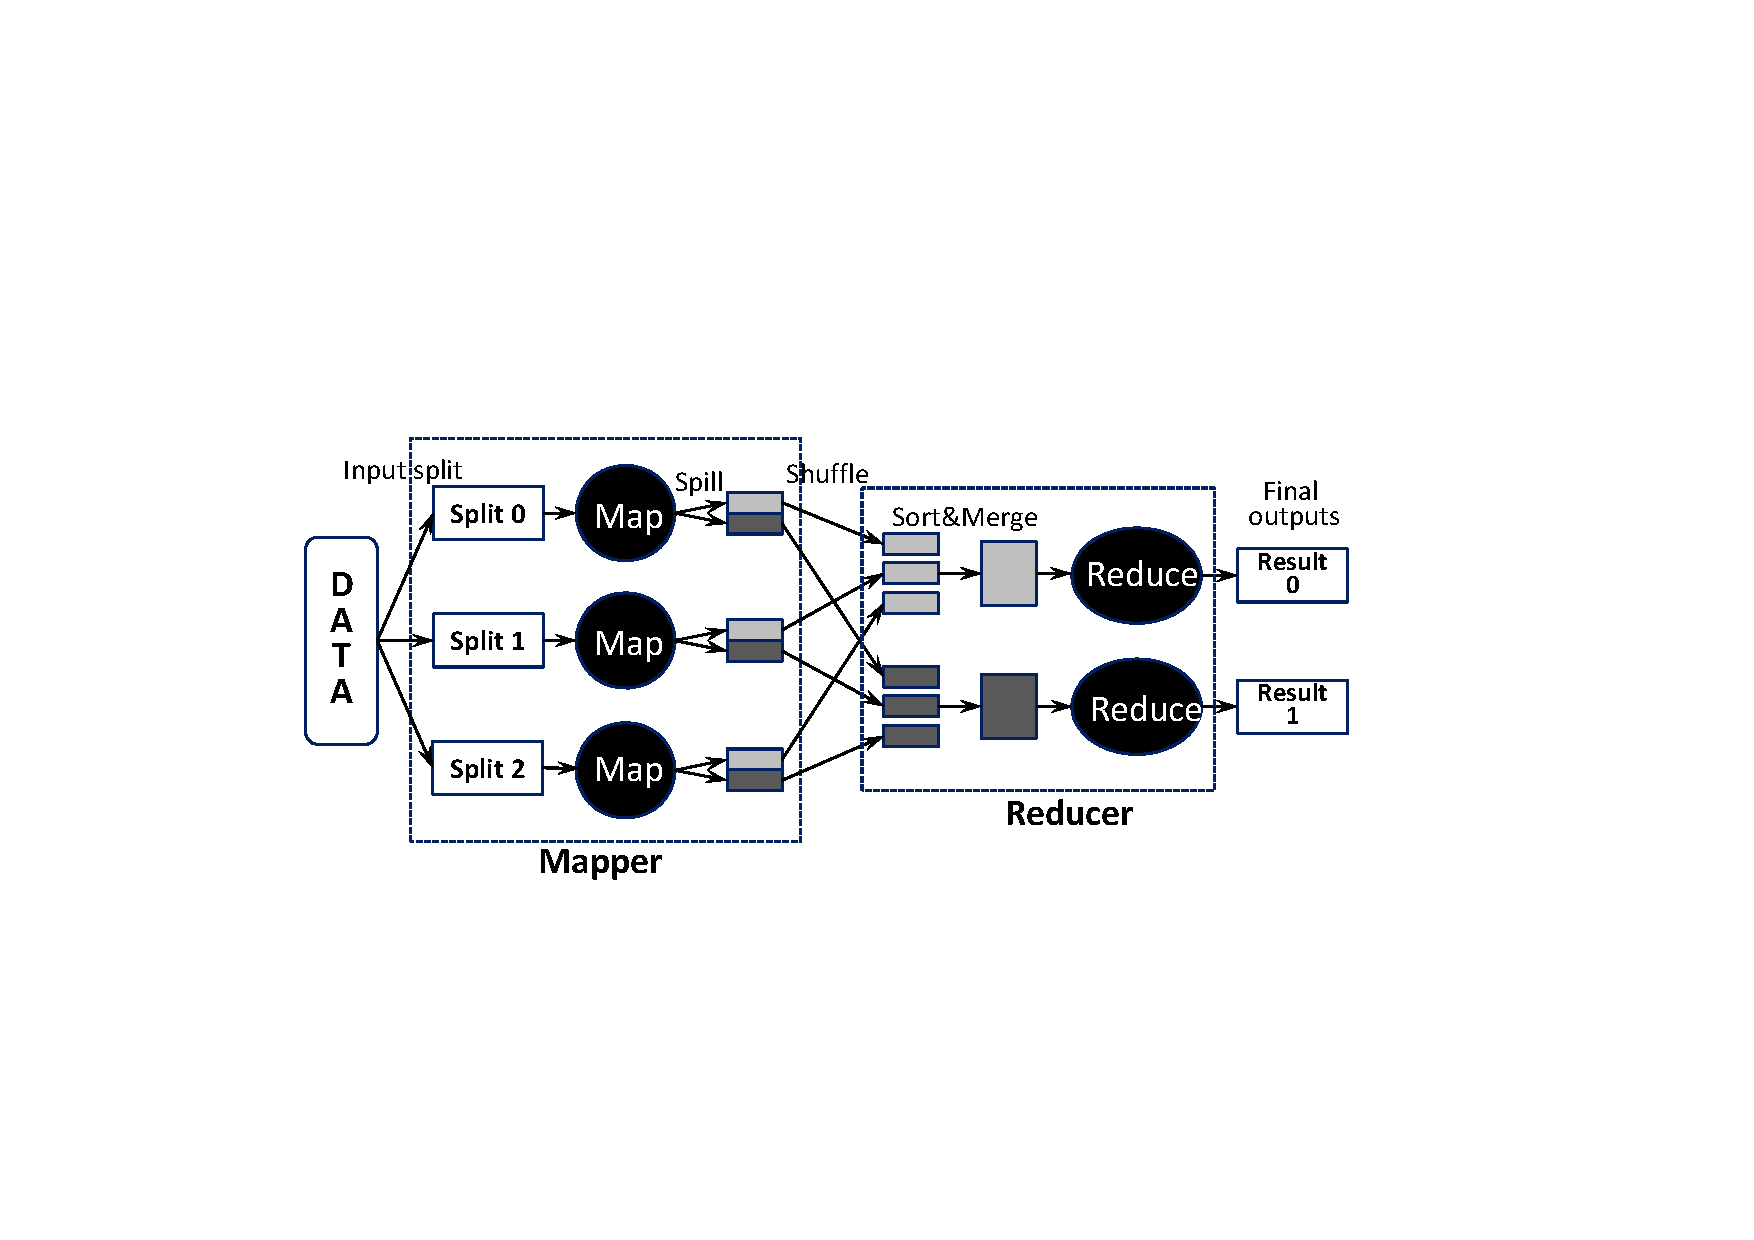
\includegraphics[width=0.99\columnwidth]{figures/HadoopMR_mono1.pdf}
 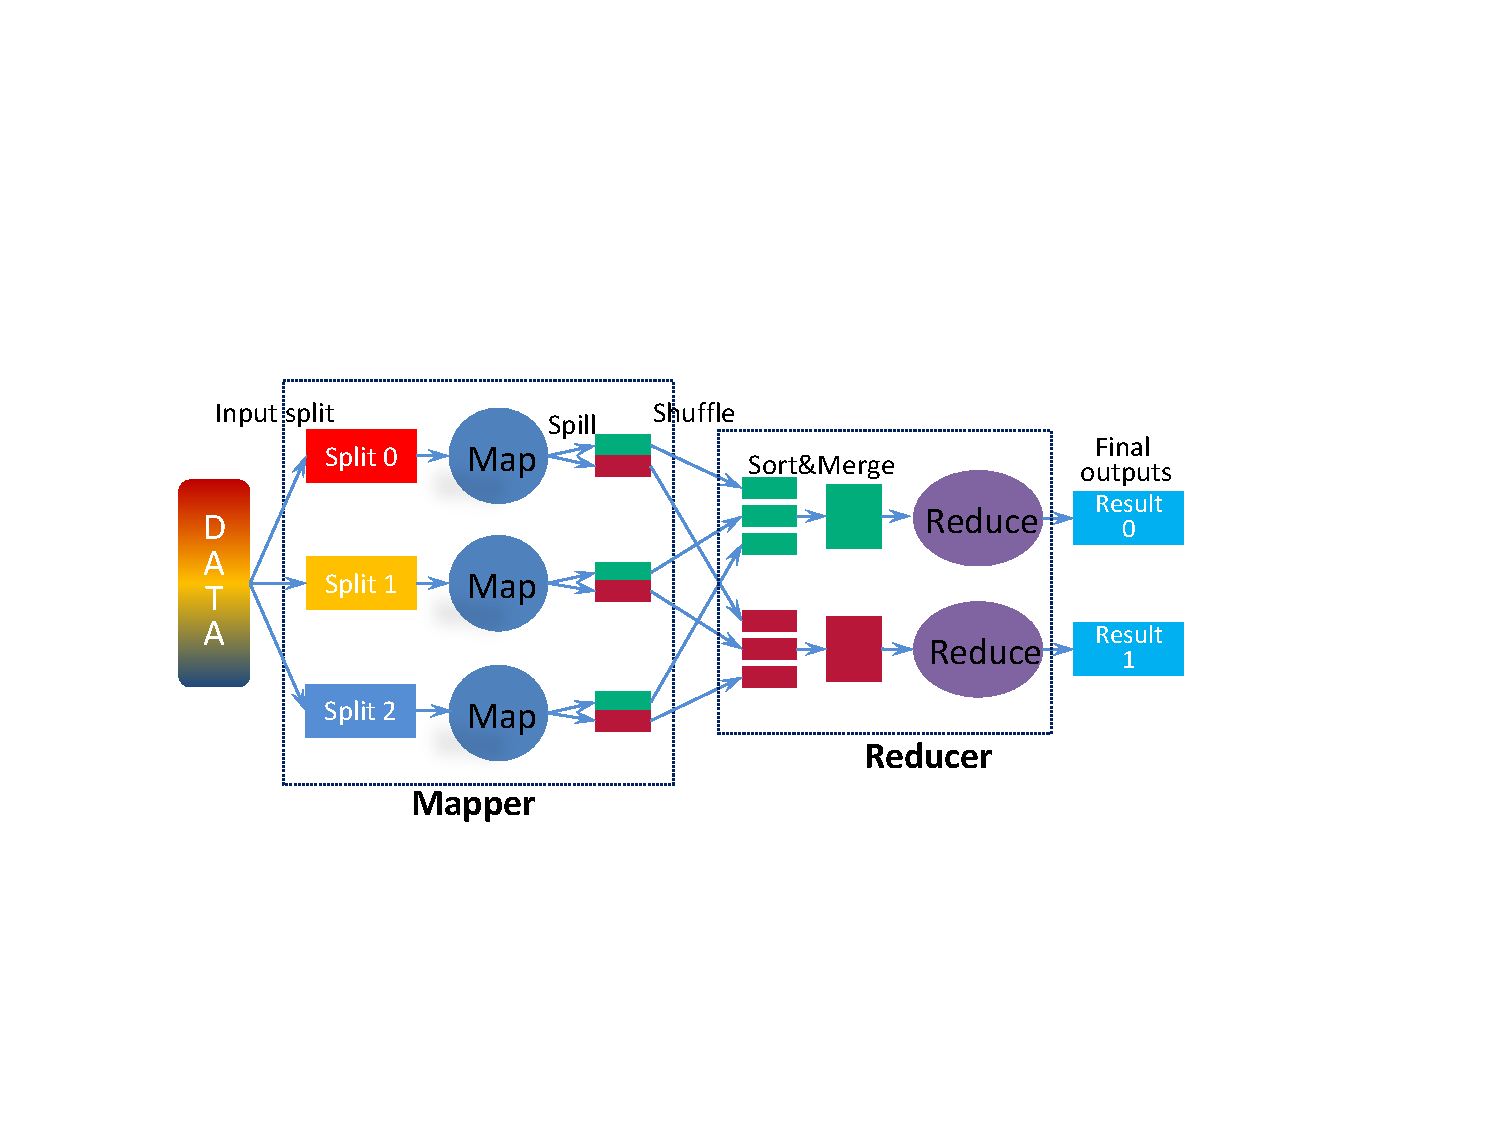
\includegraphics[width=0.99\columnwidth]{figures/HadoopMR.pdf}
\end{tabular}
  \caption{Hadoop MapReduce Framework}
  \label{fig:HadoopMR}
 \end{figure}



Hadoop is an open source implementation of the original MapReduce parallel programming model and system designed by Google~\cite{MapReduce:OSDI:2004}. MapReduce is a software framework for distributed processing of large data sets on commodity clusters~\cite{HadoopMapReduce:ACM:2010}. The Hadoop MapReduce framework leverages a distributed file system called the Hadoop Distributed File System (HDFS) which is an open source implementation of Google Distributed File System (GFS)~\cite{GFS:SOSP:2003}. The main design of the HDFS is heavily optimized for manipulating very large files with streaming data access patterns (i.e., write-once, read-many patterns). A MapReduce job consists of both Map and Reduce tasks, and one complete MapReduce job is subdivided largely into three phases: Map, Shuffle, and Reduce phase.

As illustrated in Figure~\ref{fig:HadoopMR}, at the beginning of a Hadoop MapReduce processing, Hadoop splits large input data into a set of data chunk of a predefined size (by default 64MB). Each split data is fed to each Map task which is executed in parallel on many physical machines. The Map tasks apply the Map function to its own input split data and generate a set of output data (i.e., intermediate key-value pairs). If a user implemented an optional combine function, Map tasks apply this combine function to each key-value pair list at this moment. Now, each Map task partitions the intermediate data (key-value pairs) into the number of Reduce groups. 
We offload this Map function into the ISC device.

Once all Map tasks are successfully completed, Hadoop MapReduce framework transfers the Map outputs to the Reducers as inputs, which is known as the Shuffle. Each Reduce task requests one intermediate data file from each Map task and starts to merge them on the basis of the intermediate key. Someone think of this Shuffle phase simply as a part of Reduce phase and they call it a 'copy' step in the Reduce phase.

After all Reduce tasks copy their own intermediate data, they start to sort and merge them first. Then they apply a Reduce function to the sorted data and emit the final output for each Reducer. Reduce tasks write their final outputs to a file with Hadoop Distributed File System (HDFS).






%\textcolor{red}{Need more description on namenode, datanode, job tracker and task tracker.}

%\textcolor{red}{For general search engines, many other techniques, e.g., caching, early termination. These works are orthogonal to us. We can also benefit from that.}

